\section{Algorytm genetyczny hybrydowy}

\subsubsection{Kod źródłowy}

\begin{figure}[H]
	\centering
	\hspace*{-0.8in}
	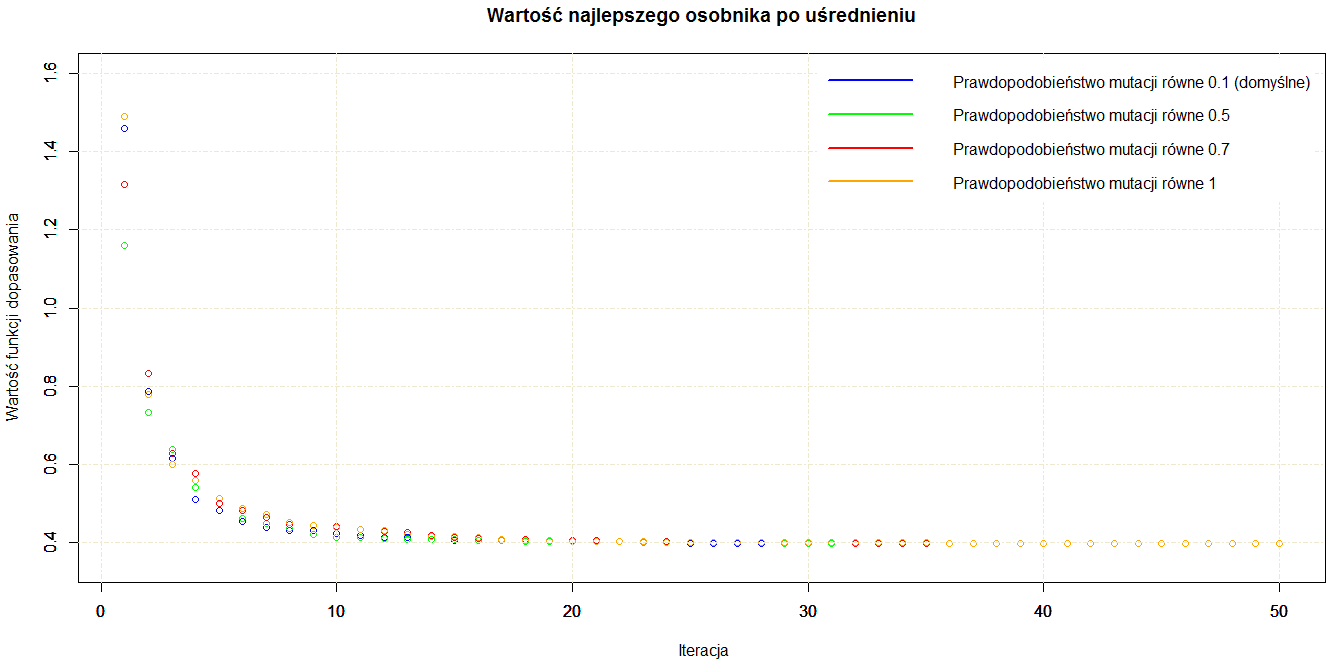
\includegraphics[scale = 0.5]{zad3_mut_max}
	\caption{!!!}  
	\label{rys:zad3_mut_max} 
\end{figure}

\begin{figure}[H]
	\centering
	\hspace*{-0.8in}
	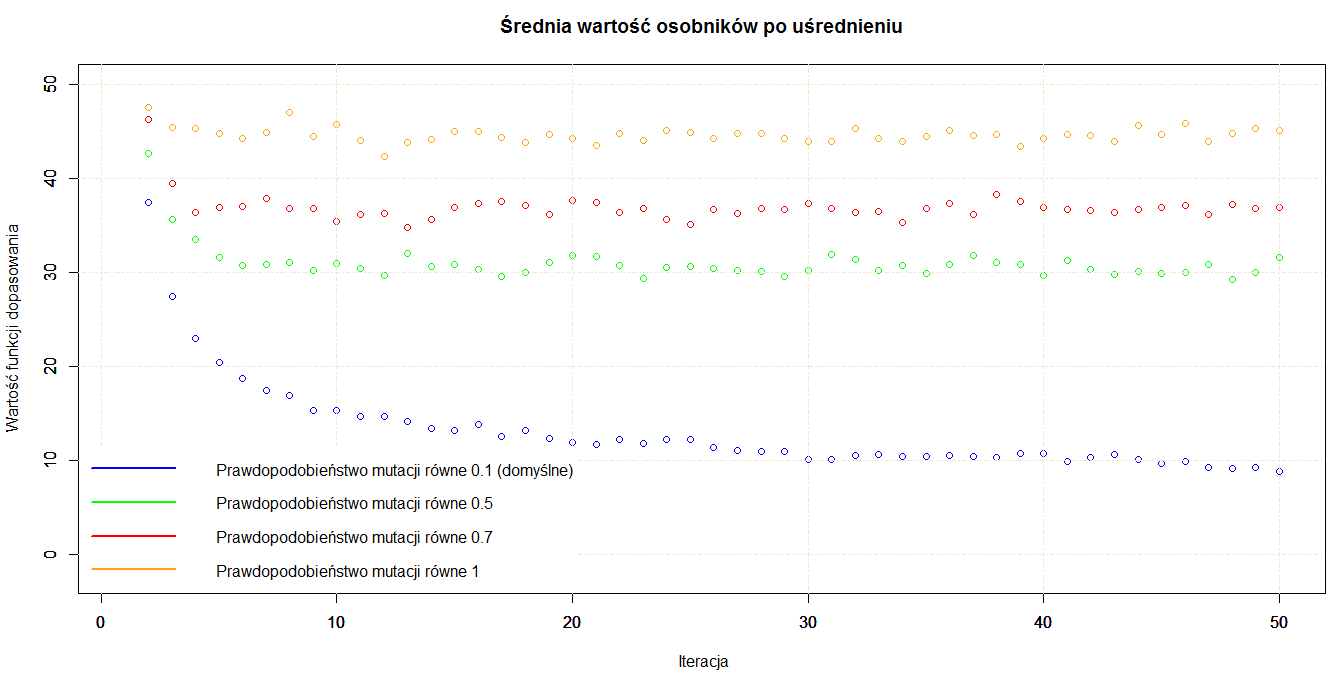
\includegraphics[scale = 0.5]{zad3_mut_mean}
	\caption{!!!}  
	\label{rys:zad3_mut_mean} 
\end{figure}

\begin{figure}[H]
	\centering
	\hspace*{-0.8in}
	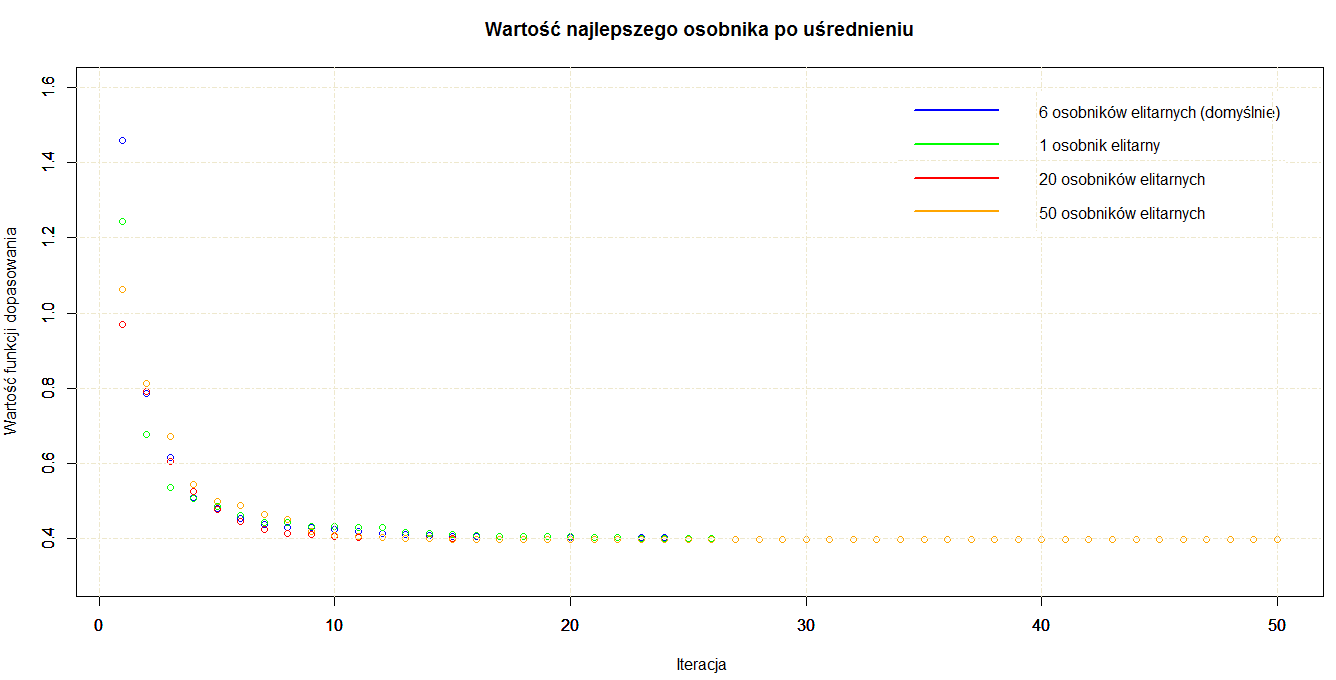
\includegraphics[scale = 0.5]{zad3_sel_max}
	\caption{!!!}  
	\label{rys:zad3_sel_max} 
\end{figure}

\begin{figure}[H]
	\centering
	\hspace*{-0.8in}
	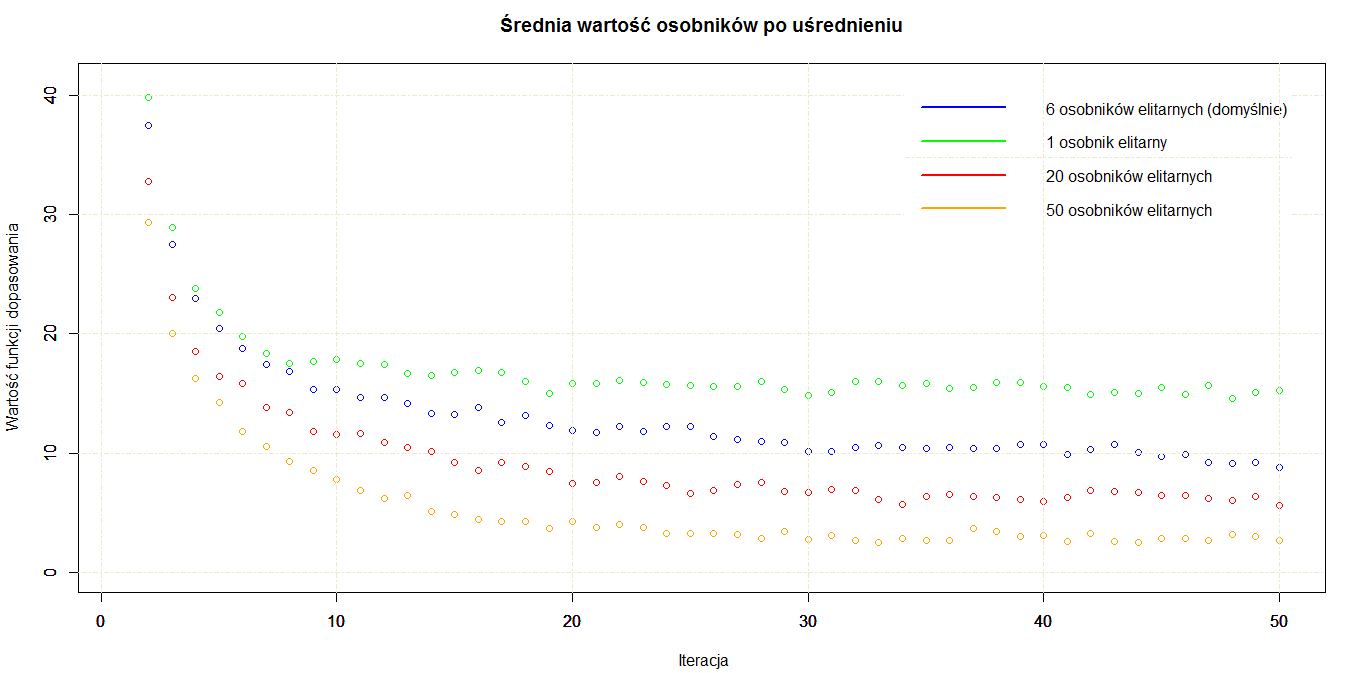
\includegraphics[scale = 0.5]{zad3_sel_mean}
	\caption{!!!}  
	\label{rys:zad3_sel_mean} 
\end{figure}

\subsubsection{Wyniki badań}


1. Wartości domyślne

> round(tail(meanRowsMean, n=1), digit=6)
[1] 8.811131
> round(tail(meanRowsMax, n=1),  digit=6)
[1] 0.398058


2. mut = 0.5

> round(tail(meanRowsMean, n=1), digit=6)
[1] 31.62451
> round(tail(meanRowsMax, n=1),  digit=6)
[1] 0.397912


3. mut = 0.7

> round(tail(meanRowsMean, n=1), digit=6)
[1] 36.9159
> round(tail(meanRowsMax, n=1),  digit=6)
[1] 0.39793


4. mut = 1

> round(tail(meanRowsMean, n=1), digit=6)
[1] 45.09641
> round(tail(meanRowsMax, n=1),  digit=6)
[1] 0.398302

---------------------------------

1.sel=1

> round(tail(meanRowsMean, n=1), digit=6)
[1] 15.28275
> round(tail(meanRowsMax, n=1),  digit=6)
[1] 0.398001

2.sel=20

> round(tail(meanRowsMean, n=1), digit=6)
[1] 5.619913
> round(tail(meanRowsMax, n=1),  digit=6)
[1] 0.397887

3.sel=50

> round(tail(meanRowsMean, n=1), digit=6)
[1] 2.657782
> round(tail(meanRowsMax, n=1),  digit=6)
[1] 0.397887


\subsubsection{Wnioski}

\begin{table}[!h]
	\hspace*{-1.5in}
	\centering
	\caption{Wartości średnie i najlepsze osobnika dla domyślnej i własnej funkcji mutacji}
	\label{mut_porownanie}
	\hspace*{-0.4in}
	\begin{tabular}{|c|c|c|c|c|}
		\hline
		\textbf{Prawdopodobieństwo} & \multicolumn{2}{c}{\textbf{Mutacja domyślna}}  & \multicolumn{2}{|c|}{\textbf{Mutacja własna}} \\ \cline{2-5}
		\textbf{mutacji} & Wartość średnia & Najlepszy wynik & Wartość średnia & Najlepszy wynik \\ \hline
		
		0.1 & 5.753710  & 0.398006 & 0.398736 & 0.398687 \\
		0.5 & 31.029570 & 0.401904 & 0.415733 & 0.398201 \\
		0.7 & 38.184020 & 0.404532 & 0.567679 & 0.398926 \\
		1   & 46.920430 & 0.408154 & 0.452637 & 0.400847  \\ \hline      
	\end{tabular}
\end{table}
